\documentclass[a4paper,12pt]{article}
\usepackage{amsmath}
\usepackage{graphicx}
\usepackage[margin=1in]{geometry}
\begin{document}

\title{Introduction to derivatives, light and energy}
\maketitle
\section{Derivatives of polynomials }

Note that the derivative of a constant is zero, as a rule. Let $a,b$ be real numbers.
\begin{enumerate}
	\item{Expand $(ax+b)^2$}
	\item{Calculate the derivate of the result.}
	\item{Simplify your answer by removing common factors from the terms.}
	\item{Take the derivate of $ax+b$}
	\item{Compare your results from 4 and 3. Can you guess what the rule is for taking derivatives of brackets?}
\end{enumerate}

\section{Graphing}

\begin{enumerate}
	\item{Sketch the graph of the function $f(x) = (x^2 - 1)(x+1)$. Note the location of the roots.}
	\item{Expand the function and take the derivative of the expansion.}
	\item{Find the local minima and maxima by letting the derivative equal to zero and solving for x. Do the results line up with your sketch?}
\end{enumerate}
		

\section{Energy, light, and matter}

The 'absorption wavelength' (meaning the wavelength of light that would be absorbed by water, is 2.87 micrometres. Note the image below of the electromagnetic spectrum. 

\begin{figure}[htbp]
	\centering
	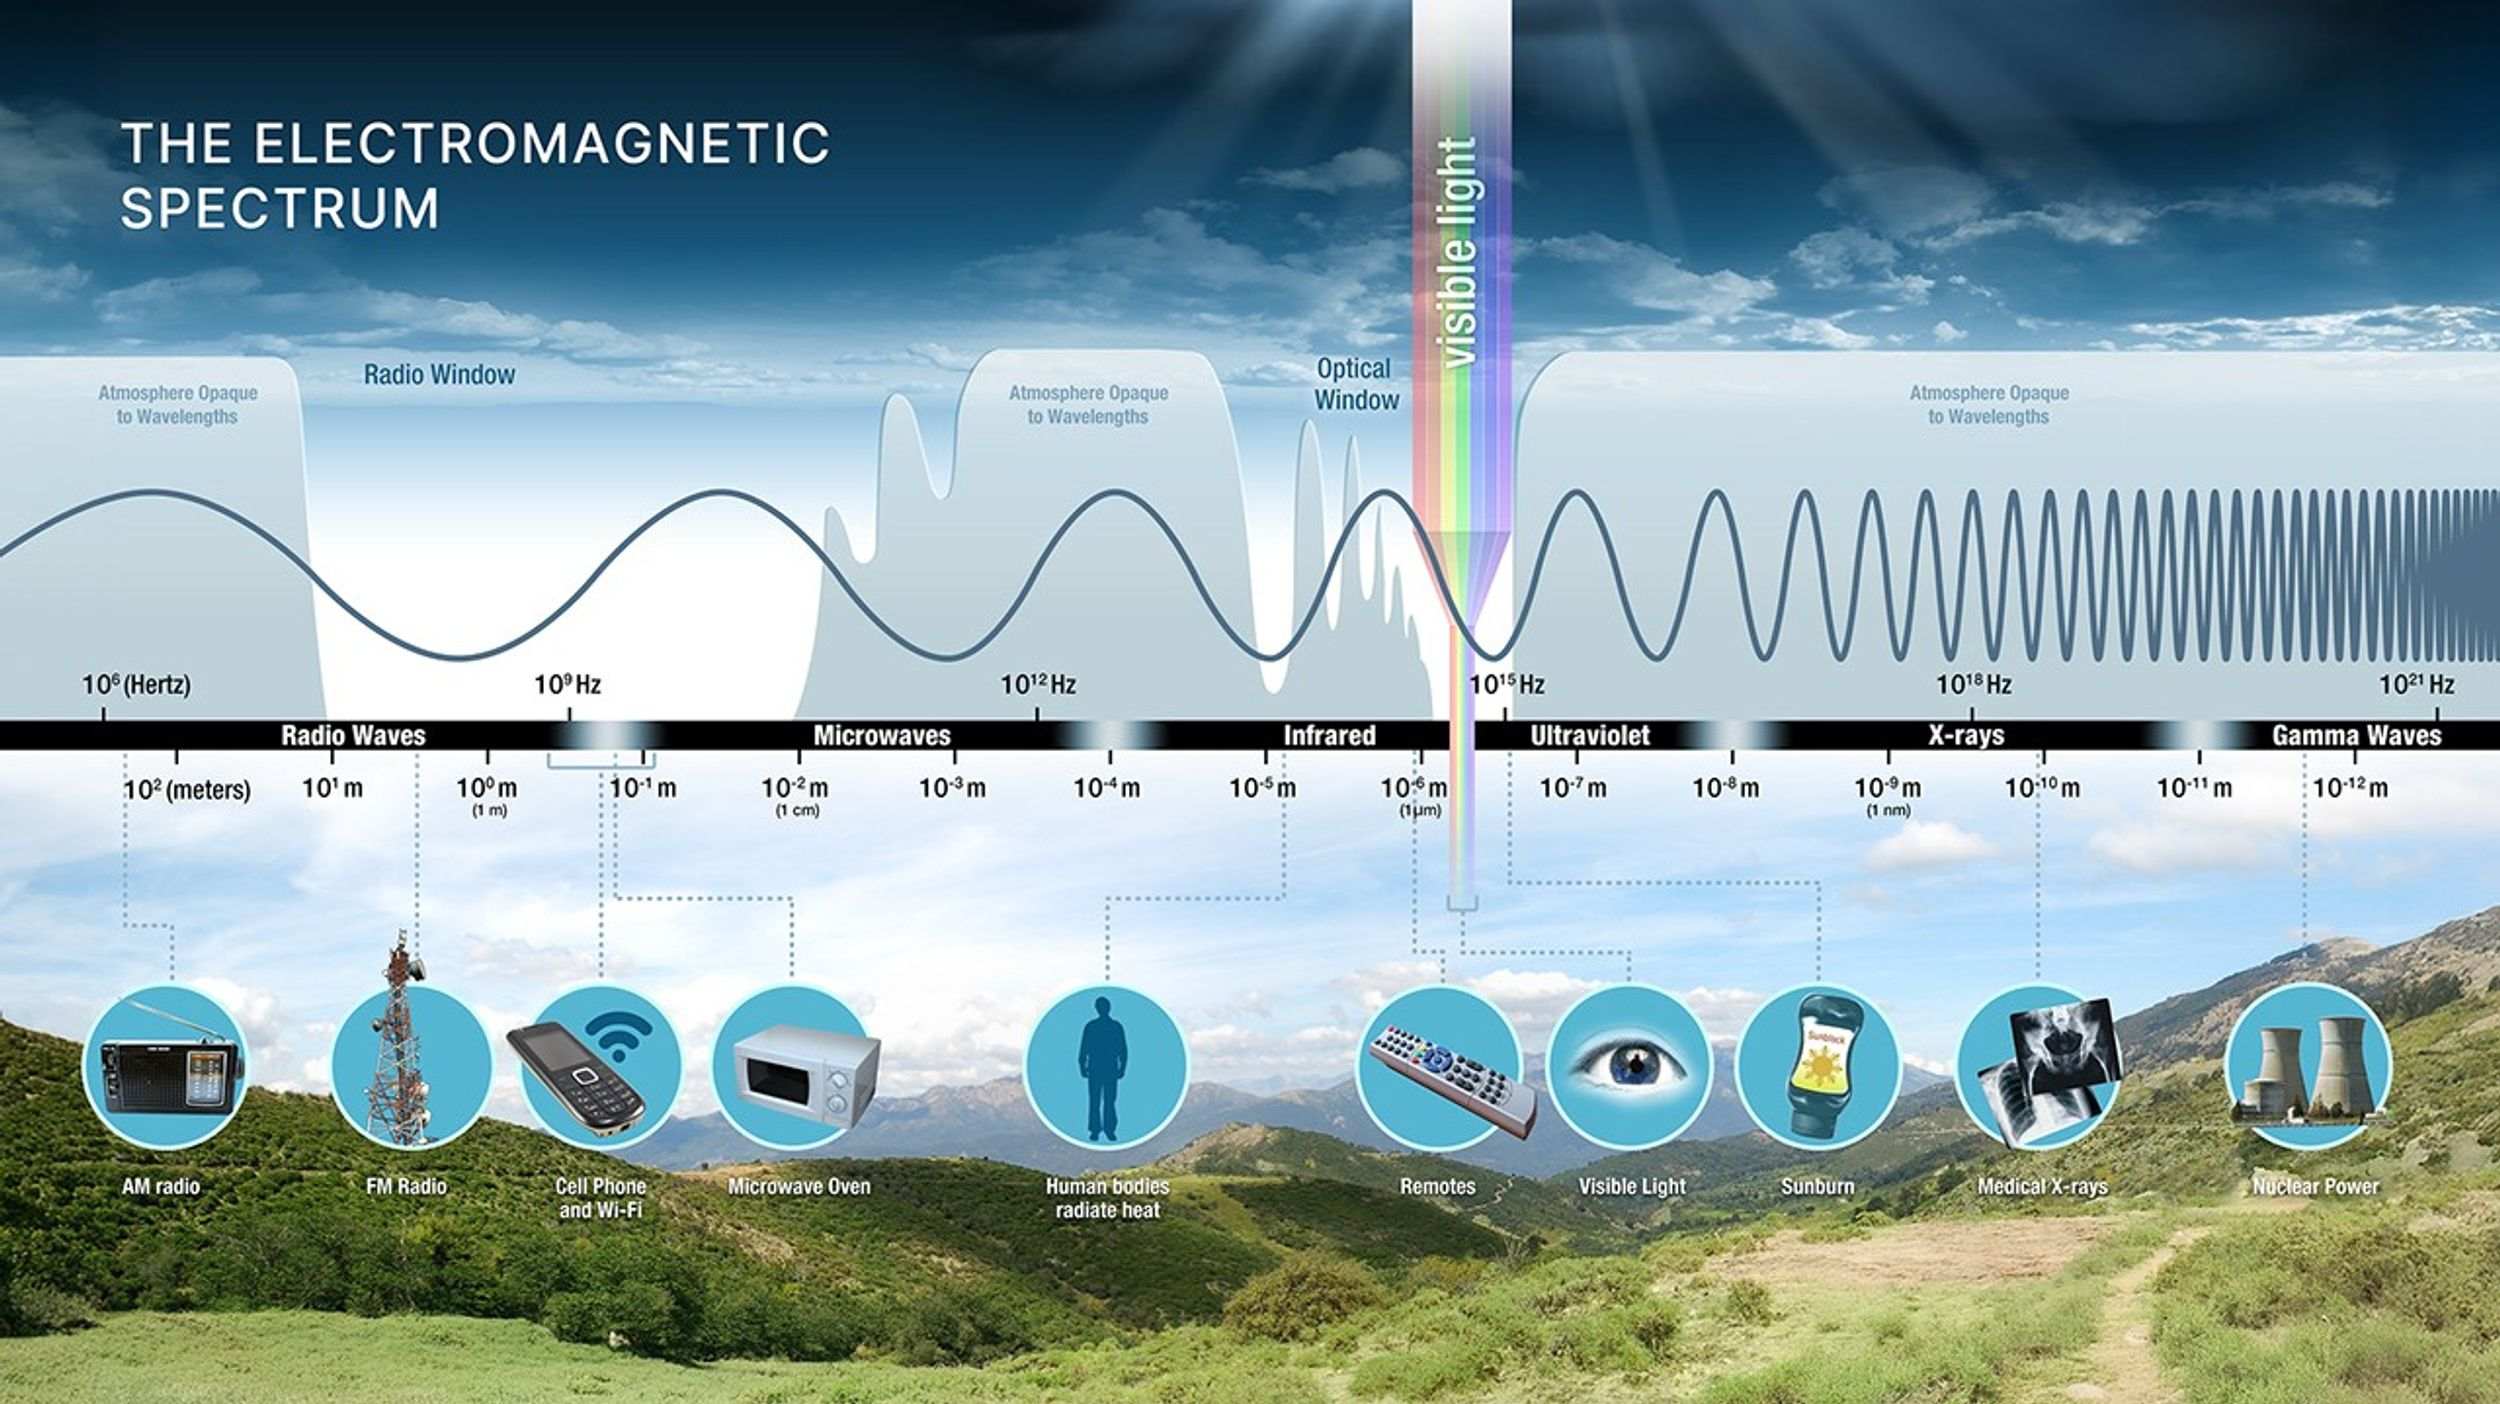
\includegraphics[angle=-90,width=1.0\textwidth]{EMS_Diagram.jpg}
	\caption{EM Spectrum}
	\label{NASA: 2026}
\end{figure}

Where does 2.87 micrometres appear on the spectrum?
\\
The typical absorption wavelength of glass is 320nm. Where does 320nm appear on the spectrum? What type of light? A microwave oven emits light at a wavelength of 12.2cm. Explain why a glass bowl filled with water would heat the water much faster than the glass itself. This is why you can remove hot food from the microwave without burning yourself (to a point).



\end{document}
